\section{Aufgabe 66}
\setcounter{section}{66}

Siehe Aufgabensammlung.

\begin{enumerate}[1.]
    \item Zeichnen Sie f"ur beide Datens"atze ein Streudiagramm der Punkte.
        \vspace{-10px}
        \begin{figure}[h]
            \centering
            \begin{minipage}[b]{0.45\textwidth}
                \centering
                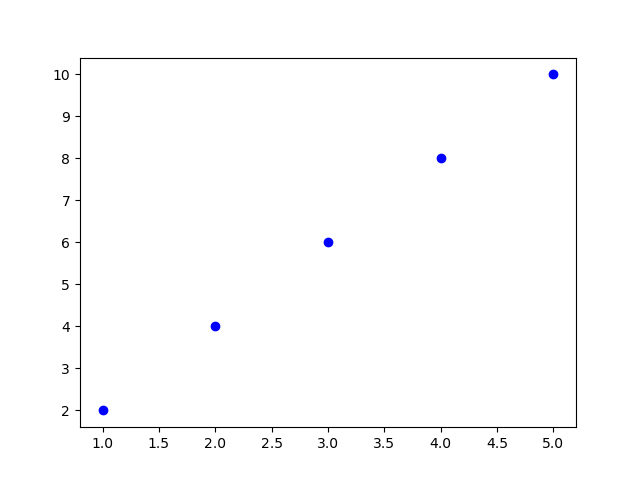
\includegraphics[width=\textwidth]{./assets/abbildung-66-1.png}
                \caption{}
            \end{minipage}
            \hspace{20px}
            \begin{minipage}[b]{0.45\textwidth}
                \centering
                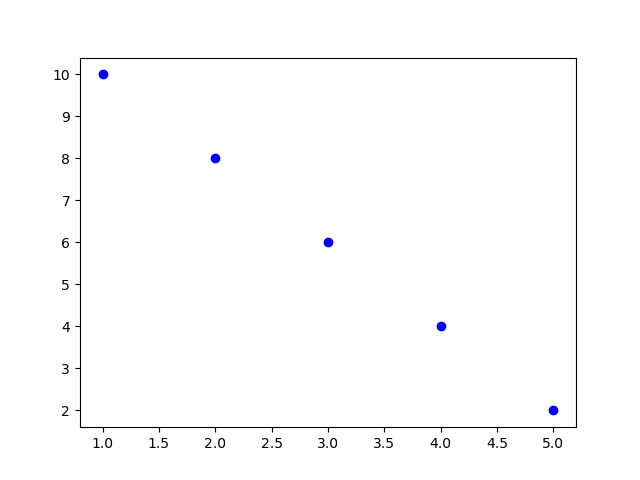
\includegraphics[width=\textwidth]{./assets/abbildung-66-2.png}
                \caption{}
            \end{minipage}
        \end{figure}
    \item Berechnen Sie die empirische Kovarianz.
        \begin{enumerate}
            \item $s^2_x = 10$, $s^2_y = 40$, $s^2_{xy} = 4$
            \item $s^2_x = 10$, $s^2_y = 40$, $s^2_{xy} = -4$
        \end{enumerate}
    \item Berechnen Sie den Korrelationskoeffizienten.
        \begin{enumerate}
            \item $r_{xy} = 1$
            \item $r_{xy} = -1$
        \end{enumerate}
\end{enumerate}
